\chapter{Introduction to Machine Learning Toolkits}
\label{chp:Toolkits}
We have used two state-of-the-art machine learning toolkits in our project, to help us achieve our goals. These tools are:-
\begin{itemize}
    \item Intel OpenVINO computer vision toolkit
    \item Tensor Virtual Machine (TVM)
\end{itemize}
Both these tools have the same high level goal, that being the deployment of pre-trained CNN models on different hardware platforms such as CPU, GPU, FPGA etc. thereby making the high level deep learning frameworks such as Tensorflow, Caffe etc. independent of the underlying hardware. However, none of these tools alone can achieve our goals, making it necessary to use a combination of both, using certain components and features in each toolkit. Both Intel OpenVINO and TVM are described in detail in the next sections.  

\section{Intel OpenVINO}


Intel OpenVINO is an open source toolkit from Intel that allows the deployment of pre-trained deep neural networks on different hardware platforms such as CPU, GPU, FPGA, etc. The toolkit is available for installation for the Windows operating system as well as selected Linux distributions. All of the tool's libraries and plugins except the FPGA plugin are a part of the open source GitHub repository.
The functionality of OpenVINO is divided among its components, Model Optimizer and Inference Engine. This is shown in Figure \ref{fig:OpenVINO_workflow} and explained below. 
\begin{figure}[!hbpt]
    \centering
    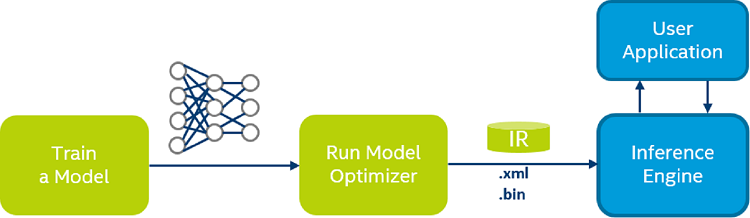
\includegraphics[width=0.65\textwidth]{img/openVINO_workflow.png}
    \caption{Intel OpenVINO workflow \citep[][]{openvino_fig}}
    \label{fig:OpenVINO_workflow}
\end{figure} 

\subsection{Model Optimizer}
The Model Optimizer is a python based tool which takes as input a pre-trained model. It supports many popular deep learning frameworks such as TensorFlow, Caffe, PyTorch, MXnet, etc. This model is then converted to a common intermediate format (IR), thereby making the inference engine independent of the training framework. The IR contains a .xml file which represents the computational graph of the CNN and a .bin file containing the weights. The graph is optimized by fusing different layers of the original topology wherever possible. Typically the batch normalization layers are fused with their preceding convolution layer and the convolution filter weights are accordingly adjusted. The toolkit comes with a model downloader which can download various openly available pre-trained models for different frameworks.
 

 \subsection{Inference Engine}
 The Inference Engine is responsible for the execution of the model on the selected hardware. For this purpose, it provides a C++ API which can be integrated into an application. The main task performed by the inference engine is to read the intermediate representation of the model, select the hardware for deployments such as CPU or FPGA and call the appropriate plugin which defines all necessary data structures and functions required to perform inference and return the output along with performance statistics. 
 The toolkit comes with pre-compiled bitstreams for a few supported FPGA boards. These bitstreams implement various popular network topologies such as GoogLeNet, ResNet, etc. as well as generic layers which are used to program the FPGAs as per the requirement of the given model topology.
 
 These bitstreams however, do not support the Intel Stratix 10 FPGA boards available in the Noctua infrastructure. In addition to this, the FPGA plugin of the inference engine is not open source, making it infeasible to use OpenVINO as a stand alone tool to achieve our project goals without customizing its components at the source code level.
 
 \subsection{OpenVINO source code}
 The Intel OpenVINO toolkit is open source and the code is available as a Github repository known as Deep Learning Deployment Toolkit (DLDT). The repository contains source code for both the Model Optimizer as well as the Inference Engine except for the FPGA plugin. As a result, we have written our own FPGA plugin for OpenVINO to support the Noctua infrastructure and enable scaling of CNNs over multiple FPGAs. 
 
 \subsection{FPGA plugin}
 The main purpose of the FPGA plugin is to flash the bitstreams (.aocx files) for the CNN models on the FPGAs and to launch the kernels according to the CNN topology. It also supports scaling on multiple FPGAs which has been achieved through the use of MPI (Message Passing Interface) and the serial I/O channels present between FPGA nodes in the Noctua infrastructure. 
 
 The plugin interacts with the Inference Engine C++ API which helps in parsing the intermediate representation obtained from the model optimizer for a given CNN model. We have reused the classes and data structures in this API as much as possible, specifically for parsing the .xml file in the IR containing the topology for the given CNN model, parsing the weights in the binary (.bin) file as well as parsing the input images. We have stored all the parsed information from the IR in a C++ struct for each layers. The definition of the struct is shown in the code snippet Code \ref{code:struct}.
 \begin{code}[!htb]
 \begin{minted}{c++}
 /**
 * Data structure to store information of each layer
 */
struct layersDetails
{
	//Layer ID
	int layerID;
	// Layer Name
	std::string layerName;
	//Type of Layer
	std::string layerType;
	//Pointer to the Layer Bias vector
	float *layerBias;
	//Pointer to the Layer Weights vector
	float *layerWeights;
	//Total number of biases
	int num_biases;
	//Total number of weights
	int num_weights;

	//Hashmap for parameters ( kernel, padding,dilation,precision) with its values.
	std::map<std::string, std::string> params;
	//Vector of parent layers
	std::vector<std::string> inputLayerNames;
	//Vector of child layers
	std::vector<std::string> outputLayerNames;
	//Vector of pointers to the Layers Details Structure of Children nodes
	std::vector<struct layersDetails *> children;
	//Vector of pointers to the Layers Details Structure of parent nodes
	std::vector<struct layersDetails *> parents;

	// Buffer index of the output
	int layerOutBufferIndex = 0;
	// vector of buffer index
	std::vector<int> parentOutBufferIndex;
	// Output dimension
	int outH = 0, outW = 0, outDepth = 0;
	//Flag to check if layer is executed.
	int visited = 0;
};

    
\end{minted}
\caption{Struct to store parsed IR information for each layer in CNN}
\label{code:struct}
\end{code}
 
 In addition to this pre-existing source code, we have written our own tree data structure in the plugin, to represent the CNN topology in a suitable pointer structure that adequately models the input output relationships between CNN layers, thus allowing us to launch their corresponding OpenCL kernels in an orderly fashion. 
 
 The plugin also supports scaling over multiple FPGAs, through the use of MPI and dedicated serial I/O connections between FPGA boards that are present in the Noctua infrastructure. The infrastructure consists of 16 FPGA nodes, each hosting 2 Intel Stratix 10 FPGA boards. Our plugin has multiple instances running as MPI processes, one per node. Each plugin instance is thus responsible for the execution of partial CNN topology on 2 FPGAs. We divide the CNN model at the OpenCL level into multiple .cl files which are then synthesized to generate their corresponding bitstreams. These bitstreams are then named in a suitable fashion so as to create a mapping between them and the specific plugin instance running on a FPGA node which is identified by its MPI rank. To map the names of the CNN layers (OpenCL kernels) to the .aocx file that contains them, we use Intel OpenCL SDK binutils to generate a .xml file corresponding to each .aocx bitstream. The plugin instance would thus flash appropriate .aocx files according to its MPI rank and then launch appropriate kernels that are contained in those .aocx files, after parsing the corresponding xmls. 
 
 The sequence diagram in the Figure \ref{fig:plugin_uml} shows the operations during the execution of the plugin.
 \begin{figure}[!hbpt]
    \centering
    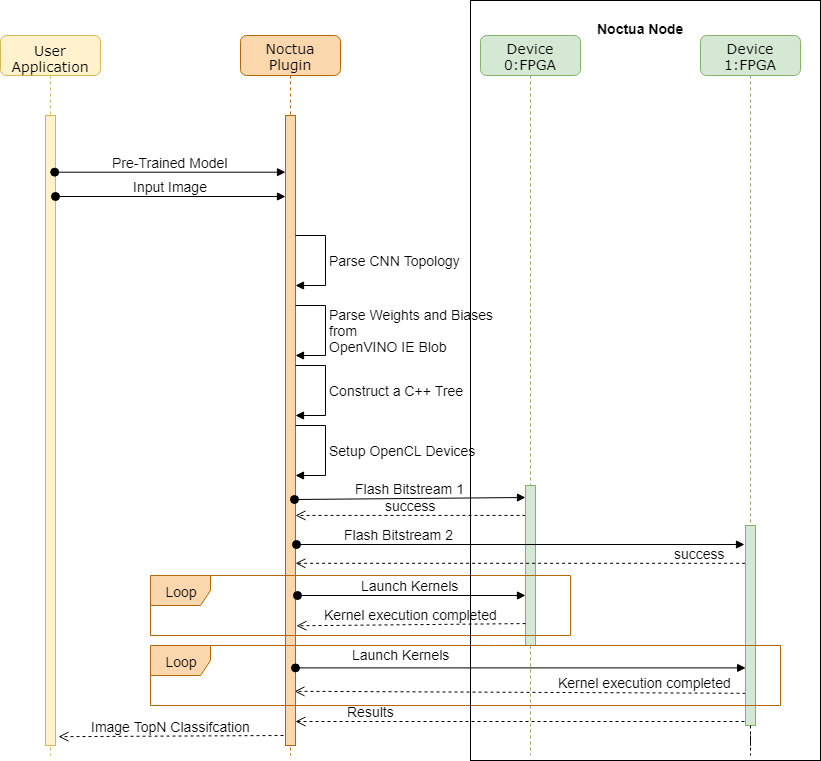
\includegraphics[width=\textwidth]{img/Plugin_UML_1.png}
    \caption{Sequence diagram of the Inference Engine at one node}
    \label{fig:plugin_uml}
\end{figure} 

 \begin{itemize}
     \item The user application sends the CNN model IR and the input image to the plugin.
     \item The FPGA plugin parses the IR, both the xml and bin files to retrieve the layer information and the weights which are then used to construct a tree data structure.
     \item The plugin instance then flashes the appropriate bitstreams on the FPGA boards and parses their corresponding xml files to get a mapping between the aocx files and the kernel names.
     \item The kernels are then launched by a level wise traversal of the tree structure representing the CNN model.
     \item One instance of the plugin is executed parallelly at every node.
     \item The plugin instance at the last node collects results and returns them to the user application which displays the top N labels and their softmax scores (confidence) to the user.
 \end{itemize}
 
 \subsection{Advantages}
  
 \begin{itemize}
 \item Supports optimization of models and quantization of weights.
 \item A CNN model can be deployed on hardware with minimal programming effort and independent of the training framework.
 \item For FPGAs, the use of pre-compiled bitstreams eliminate the time needed for synthesis of kernel codes.
 \end{itemize}
 
 \subsection{Disadvantages}
 \begin{itemize}
 \item The main disadvantage is the compatibility of FPGA boards. Development and synthesis of kernel codes along with a plugin for FPGAs may be required to make OpenVINO work with unsupported boards. 
 \item Scaling to multiple FPGAs, which is one of the goals of this project is non-trivial as it would require the development of overlays for external I/O channels. 
 \end{itemize}
\section{TVM}
Due to extensive research in the field of machine learning especially in Image recognization and object detection largely due to competition such as ILSVRC (Imagenet Large scale visual recognization challenge), there is a demand and need for developing hardware specific to increased computation capabilities and caching mechanisms. Various computational superior hardware such as CPU, GPU, and accelerators such as ASICs and FPGA are been used to deploy Machine Learning (ML) models and to draw the inference. To build and deploy such ML models we use Deep learning (DL) frameworks such as Tensorflow, Caffe, MXNET, Keras, etc. There is extensive support and libraries available for CPUs and certain vendor-specific GPUs. But for accelerators, there is limited support and libraries available which makes it difficult and tedious to deploy ML models on them.  We use Tensor Virtual Machine (TVM) an open-source compiler and code generator which addresses “graph level and operator level optimizations” \cite{tvm_fig}. TVM supports a wide range of hardwares and accelerators. 

There are two types of optimizations that can be carried out during code generation for a DL model, high-level optimizations where graph and operators of the model are optimized and low-level optimizations where low-level programs are  optimized with respect to specific hardware architecture.
Each hardware has its own memory architecture, data operators and dataflow handling mechanism this diversity makes it difficult for efficient graph generation and machine code optimizations.
TVM performs high-level optimizations such as operator fusion where basic operators are fused together and also perform graph optimization where DL activation functions are fused along with convolutions or other functions. It also performs machine code optimizations based on the hardware architecture and compute primitives. TVM uses a learning-based cost model for selection of operators involved in code generation. The TVM compilation stack is shown in Figure \ref{fig:tvm_fig}.

\begin{figure}[h!]
    \centering
    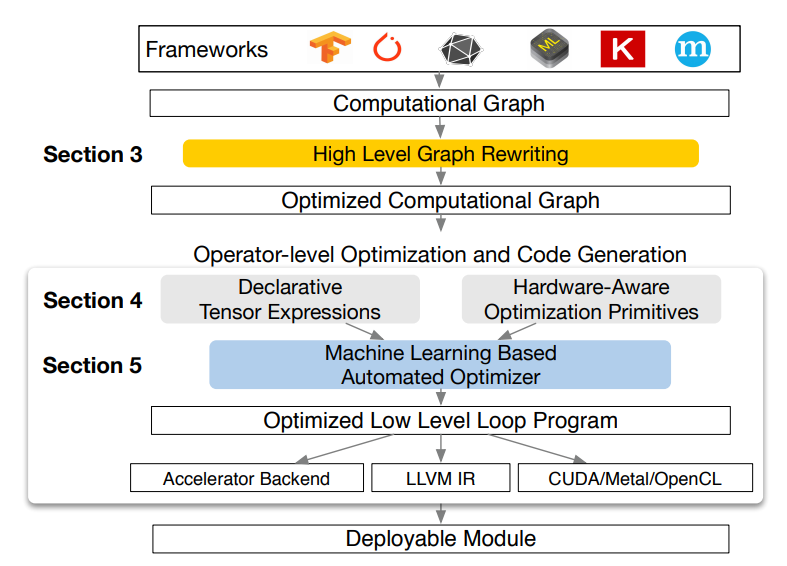
\includegraphics[scale=0.50]{tvm_overview.png}
    \caption{System overview of TVM \cite{tvm_fig}}
    \label{fig:tvm_fig}
\end{figure} 

Following Chen et al.\cite{tvm_fig} TVM performs these three steps: 
\begin{enumerate}
  \item DL frameworks take a model in the form of a frozen \textit{protobuf} file and transform it into a computational graph representation. This computational graph is provided to the TVM graph rewriter which performs graph level optimizations such as operator fusion, constant folding, static memory planning pass, and data layout transformation. These graph level optimizations are been discussed below.
  \begin{itemize}
     \item Operator Fusion - Computation graph intermediate representation (IR) stores intermediate results of certain operators before being used for further computations. TVM performs operator fusion where such operators are fused together along with its predecessor or successor operators based on the type of operator and the operations it performs to form a single kernel. TVM classifies operators into four types namely 1) injective 2) reduction 3) complex-out-fusable and 4) opaque (unfusable operators) \cite{tvm_fig}.
     \item Constant Folding - Certain graph operators have constant values that can be pre-computed during compile time instead of runtime. Thus saving resources and time during code-generation. Constant-folding is a process of finding such operators and replacing them with a constant value. In TVM, it is performed by graph rewriter which mathematically calculates the constant value for such operators and substitutes them in the graph.
     \item Static memory planning pass - Intermediate tensors (data) needs to be stored for further executions. During computational graph optimization, graph rewriter pre-allocates memory to store such tensors.
     \item Data layout transformation - Each hardware has its own data-layout choices based on various factors and memory hierarchies. The computational graph needs to match the internal data layout of the selected hardware. Graph rewriter performs data layout transformation, where it first collects the constraints and ideal data layout for the operators in the selected hardware. These constraints are based on the memory hierarchy of the hardware. Then the mapping of the data layout is performed between the selected operator and the hardware.
   \end{itemize}.
   
  \item TVM has developed \textit{tensor expression language} which provides compute operators with its computing rules and shapes. It supports arithmetic and mathematical operators which are used for computation in DL models. The key feature of this tensor expression is that it is hardware aware language which means based on the target hardware operators can be optimized to gain maximum benefit from the optimization. TVM implements a concept known as “schedule transformation” \cite{tvm_fig} by applying basic transformations on the tensor expressions in a periodic and incremental fashion. During this process, it also keeps additional information about the loop structures and data types which is used during low-level code generation.
  
  TVM implements nested parallelism using the idea of \textit{shared-nothing nested parallelism} and allowing a certain group of threads to fetch data required by them and store it in local memory for easy access. Such collaboration helps in sharing the data with its counterpart/sibling threads. For latency hiding, TVM introduces a concept called “virtual threading schedule primitive” \cite{tvm_fig} where pipeline parallelism is implemented for the target hardware by generating single instruction set from multithreaded instructions which are provided using virtual threads. The single instruction set is achieved using low-level synchronization.
  
  \item  TVM provides us with multiple implementations of the operators, selecting between these operators is based on performance of the operator implementation with respect to the selected hardware. TVM solves this problem by developing a concept called “automated schedule optimizer” \cite{tvm_fig}.
Automated schedule optimizer consists of two components:

\begin{itemize}
     \item Schedule Explorer - Creates a template configuration for the selected hardware with the help of configurable options provided by the developer.
     \item ML-Based Cost model - For the selected operator configuration, the ML model predicts the runtime of the lowered loop program from the configuration. The model training is carried out based on the runtime data collected from various configurations. As more and more configurations are provided the cost model improves its accuracy.
   \end{itemize}
\end{enumerate}


 \begin{code}[!htb]
 \begin{minted}{Python}
target = 'aocl_sw_emu'
target_host = 'llvm'
layout = 'NCHW'
ctx = tvm.cpu(0)

img_path = download_testdata(image_url, img_name, module='data')

model_path='resnet_frozen.pb'

with tf.gfile.FastGFile(model_path, 'rb') as f:
    graph_def = tf.GraphDef()
    graph_def.ParseFromString(f.read())
    graph = tf.import_graph_def(graph_def, name='')
    graph_def = tf_testing.ProcessGraphDefParam(graph_def)
    # Add shapes to the graph.
    with tf.Session() as sess:
        graph_def = tf_testing.AddShapesToGraphDef(sess,
        'resnet_v2_50/predictions/Reshape_1')   

from PIL import Image
image = Image.open(img_path).resize((224, 224))

shape_dict = {'DecodeJpeg/contents': x.shape}
dtype_dict = {'DecodeJpeg/contents': 'uint8'}

sym, params = nnvm.frontend.from_tensorflow(graph_def, layout=layout,
shape=shape_dict)


with nnvm.compiler.build_config(opt_level=3):
    graph, lib, params = nnvm.compiler.build(sym,  target=target,
    target_host=target_host,  params=params)


\end{minted}
\caption{TVM Python API code for ResNet-50}
\label{code:TVMAPI}
\end{code}


In Code \ref{code:TVMAPI}, we use TVM API to get OpenCL generated code for ResNet-50 model.
After the compilation of the program, TVM provides us with an output file with the kernels for FPGA, the optimized computation graph, the library of operators present in the graph for the target hardware (FPGA) and the parameters which contain weights and input for the model. The computational graph also provides us with intermediate representation and mapping of the code generated with its respective inputs.

\pagebreak
 
 Following are the important components of TVM.
 
 \subsection{Compilers}
 TVM provides us two types of compilers.
 
 
 \subsubsection{NNVM}
 
 Neural Network Virtual Machine (NNVM) is a compiler that implements operator and graph level optimizations provided by TVM to generate target hardware code. \textit{nnvm.top} (Tensor operator property registry) provides information about which operators can be scheduled together and performs those optimizations to produce the optimized graph.
 
 NNVM has four levels of operators :
 
 \begin{itemize}
    \item Level 1: Basic Operators - This level includes vary basic operators such as \textit{dense}, \textit{Relu}, \textit{sigmoid}, \textit{exp}, etc.
    \item Level 2: Convolutions - The operators related to convolution become part of this level. Eg. \textit{con2d}, \textit{max\_pool2d}, \textit{avg$textunderscore$pool2d}, etc.
    \item Level 3: Additional Tensor Operators - Operations that provide the additive feature to the original tensors are group together at this level. Eg- \textit{reshape}, \textit{floor}, \textit{round}, etc.
    \item Level 4: Broadcast and reductions - Operators such as \textit{sum}, \textit{mean}, \textit{max},  \textit{min} are part of the reduction level.
 \end{itemize}
 
 NNVM has following functionality:
 
 \begin{itemize}
    \item \textit{nnvm.frontend} take in the model provided by DL frameworks and generates NNVM compatible symbols and parameters (NDArray) which are used by NNVM.
    \item  \textit{nnvm.compiler} has  \textit{nnvm.build} and  \textit{nnvm.build\_config} functions.
    \item In \textit{build\_config} function we provide optimization level based on which graph and tensor optimizations are carried out.
    \item \textit{nnvm.build} function is used to make C API call for code generation with optimized computational graph (graph), target hardware (targer\_host), input parameters (param) and layout provided. 

 \end{itemize}
 
 TVM provides us with the following types of optimizations.
 
 \begin{itemize}
     \item Pass 0 \textit{SimplifyInference} -
It is usually carried out on batch normalization tensor operators.
 \item Pass 1 \textit{OpFusion} -
In \textit{OpFusion}, basic operators are fused together with the convolution layer along with the precomputation of tensor operators.
\item Pass  2 \textit{PrecomputePrune} -
In this level of optimization, the graph is pruned and the constant operators are precomputed and replaced with constant values. The values of such operators are mathematically precalculated and substituted with a constant value during kernel generation. The number of operations is reduced in a precomputed and pruned graph.
\item Pass  3 \textit{FoldScaleAxis} -
In \textit{FoldScaleAxis} algorithm, "[t]he general idea is to transform [tensor expression] to a tuple of value, axes, and scale, where the
final result satisfies [code \ref{code:TVMFoldScaleAxis}].
\begin{code}[!htb]
 \begin{minted}{Python}

 result = value
 for i, k in enumerate(axes):
    k-th dimension of result *= i-th dimension of scale
 \end{minted}
 \caption{TVM FoldScaleAxis \cite{FoldScaleAxis}}
\label{code:TVMFoldScaleAxis}
\end{code}
Then [compiler] can propagate this signal [tuple] along and fold the scale if necessary. [. . .] In order to make sure all the scale [compiler] sent out can be consumed eventually, [compiler runs] a backward 'preparation phase', which propagates the demand of the potential axes scaling back to its input" \cite{FoldScaleAxis}.
We have used this optimization level during our kernel generation.
 \end{itemize}
 
  \subsubsection{Relay}
Relay is known as NNVM {$V_2$}. It is a high-level functional IR for TVM.  Relay has 8 levels of definitions and is finely grained with extended support of \textit{Image operators}, \textit{Algorithm operators}, \textit{Temporary operators}, and \textit{dialect operators}. It distinguished between local and global variables been used.

\begin{itemize}
    \item Relay uses similar levels of optimizations as NNVM.
    \item \textit{relay.backend}  handles the backend request for relay interpreters. Various relay functions can be accessed through the \textit{relay.backend} interpreter.
    \item \textit{relay.frontend},  \textit{relay.build}  and \textit{relay.build\_config}  has similar functionality to its predecessor.
\end{itemize}

 \subsection{TOPI}
 For having quick access to the operators, TVM creates a library of its operators naming TVM Operator Inventory (TOPI). It contains a list of predefined operators that are used to compute operator declaration while generating computational graph. List of operators supported by TOPI are \textit{identity}, \textit{negative}, \textit{floor}, \textit{ceil}, \textit{abs}, etc.
 \begin{itemize}
\item \textit{topi.identity(x)} Returns with the identity value for the selected input.
\item \textit{topi.negative(x)} Returns with the negative value for the selected input.
\item \textit{topi.abs(x)}  Returns element-wise absolute value for the tensor operators.
 \end{itemize}
 
 \subsection{Codegen}
TVM maintains a subdirectory for code generation functionalities and it is placed under \path{src/codegen} and interacts with it using API calls. When we execute \textit{nnvm.compiler.build} function, a C++ API call is made to codegen library which is implemented in C++. When we execute the NNVM compiler an API call is registered under python \path{/tvm/api.py}. The functions present in \textit{api.py} are mapped to   \path{src/api/api_lang.cc} in its C++ counterpart.
 
  \begin{code}[!htb]
 \begin{minted}{c++}
 TVM_REGISTER_API("_Placeholder")
.set_body([](TVMArgs args,  TVMRetValue* ret) {
    *ret = placeholder(args[0],
                       args[1],
                       args[2]);
  });
 \end{minted}
\caption{TVM Register API for Placeholder Operation \cite{tvm_code}} 
\label{code:TVMRegisterAPI}
\end{code} 
In TVM C++ functions are made accessible to Python frontend using \textit{TVM\_REGISTER\_*}. In Code \ref{code:TVMRegisterAPI} a register call made to placeholder operation for Resnet-50 kernel generation.
 
 \begin{code}[!htb]
 \begin{minted}{c++}
 runtime::Module Build(const Array<LoweredFunc>& funcs,
                      const std::string& target) {
  std::string mode = target;
  size_t pos = mode.find(' ');
  if (pos != std::string::npos) {
    mode = mode.substr(0, pos);
  }
  std::string build_f_name = "codegen.build_" + mode;
  // the build function.
  const PackedFunc* bf = runtime::Registry::Get(build_f_name);
  CHECK(bf != nullptr)
      << "Target " << target << " is not enabled";
  runtime::Module m = (*bf)(funcs, target);
  return m;
}
\end{minted}
\caption{TVM codegen Build() function \cite{tvm_code}}
\label{code:TVMCodegen}
\end{code}

 The \textit{Build()} function looks up the code generator for the given target in the \textit{PackedFunc} registry. Code \ref{code:TVMCodegen} shows build function our target library is AOCL. To have a direct interaction between C++ and Python functions a \textit{PackedFunc} is implemented by TVM. Due to interoperability, a Python function can be easily called from C++ codebase making it a bidirectional connection. A \textit{PackedFunc} helps TVM make API calls type-erased, which removes the restriction for the function to be bound to specific input and return from C++ codebase. The inputs provided to the \textit{PackedFunc} are wrapped into \textit{TVMArgs} data type which is an internal data type of TVM and the function returned values are wrapped into \textit{TVMRetValue} data type. In Code \ref{code:TVMCodegenRegisterAPI} \textit{set\_body} is the \textit{PackedFunc} for the API. Since target hardware for our project has been set to aocl, \textit{Build()} function registers \textit{codegen.build\_aocl}.
 
  \begin{code}[!htb]
 \begin{minted}{c++}
  TVM_REGISTER_API("codegen.build_aocl")
.set_body([](TVMArgs args, TVMRetValue* rv) {
    *rv = BuildAOCL(args[0], args[1], false);
  });
\end{minted}
\caption{TVM codegen register API \cite{tvm_code}}
\label{code:TVMCodegenRegisterAPI}
\end{code}

\textit{BuildAOCL()} function generates OpenCL kernels from the lowered IR using \textit{CodeGenAOCL} class. Lowered IR provides us with target hardware IR in the form of machine code which can be used for code generation. The computational graph which is a high-level IR is converted in low-level IR during this process.

 \begin{code}[!htb]
 \begin{minted}{c++}
runtime::Module BuildAOCL(Array<LoweredFunc> funcs, std::string target_str,
                          bool emulation) {
  // Get code.
  using tvm::runtime::Registry;
  bool output_ssa = false;
  CodeGenOpenCL cg;
  cg.Init(output_ssa);
  for (LoweredFunc f : funcs) {
    cg.AddFunction(f);
  }
  std::string code = cg.Finish();
  if (const auto* f = Registry::Get("tvm_callback_opencl_postproc")) {
    code = (*f)(code).operator std::string();
  }

  // Write a .cl file.
  runtime::SaveBinaryToFile("aocl.cl", code.c_str());
\end{minted}
\caption{BuildAOCL() kernel generation \cite{tvm_code}}
\label{code:TVMCodegenBildAOCL}
\end{code}

\textit{BuildAOCL()} function parses through \textit{loweredFunc} and stores the code in \textit{aocl.cl} file. Fig 6.7 shows functionality of \textit{BuildAOCL()}

 \subsection{VTA}
TVM has a DL accelerator for FPGAs and GPUs in the form of Versatile Tensor Accelerator (VTA). VTA is an open-source hardware and can be customized according to the needs and requirements for various DL accelerators. FPGAs support streamlined workflow models, to make deployments of such models fluent VTA provides support for streamlined architecture. Dense linear algebra is one of the important aspects of DL. VTA performs computations such as dense linear algebra using RISC processors thus reducing the execution time and increasing the efficiency at the same. VTA has four modules namely fetch, load, compute and store module. The channel of communication between these modules is through local memory blocks (SRAM) and FIFO queues. Due to the FIFO queues, task parallelism is maintained between these modules.
\begin{itemize}
\item \textit{Fetch Module} – Instruction set needs to be loaded for computation from global memory (DRAM) and also needs to be decoded for routing them to the proper command queue. Fetch module performs those operations on the instruction set.
\item \textit{Load Module} - Once the instruction set is loaded into the module there respective input data and weights need to be loaded from DRAM and are allocated onto on-chip memory.
\item \textit{Compute Module} – Compute module is where all the computations happen for VTA. It uses General Matrix Multiplication (GEMM) to compute dense linear algebra. VTA processors require its data into register file and micro-op kernels into the micro-op cache for further processing, compute module performs those operations of loading of data from DRAM and micro-op kernels.
\item \textit{Store Module} – Stores results from \textit{compute module} into DRAM.
 \end{itemize}
 
 \begin{figure}[h!]
    \centering
    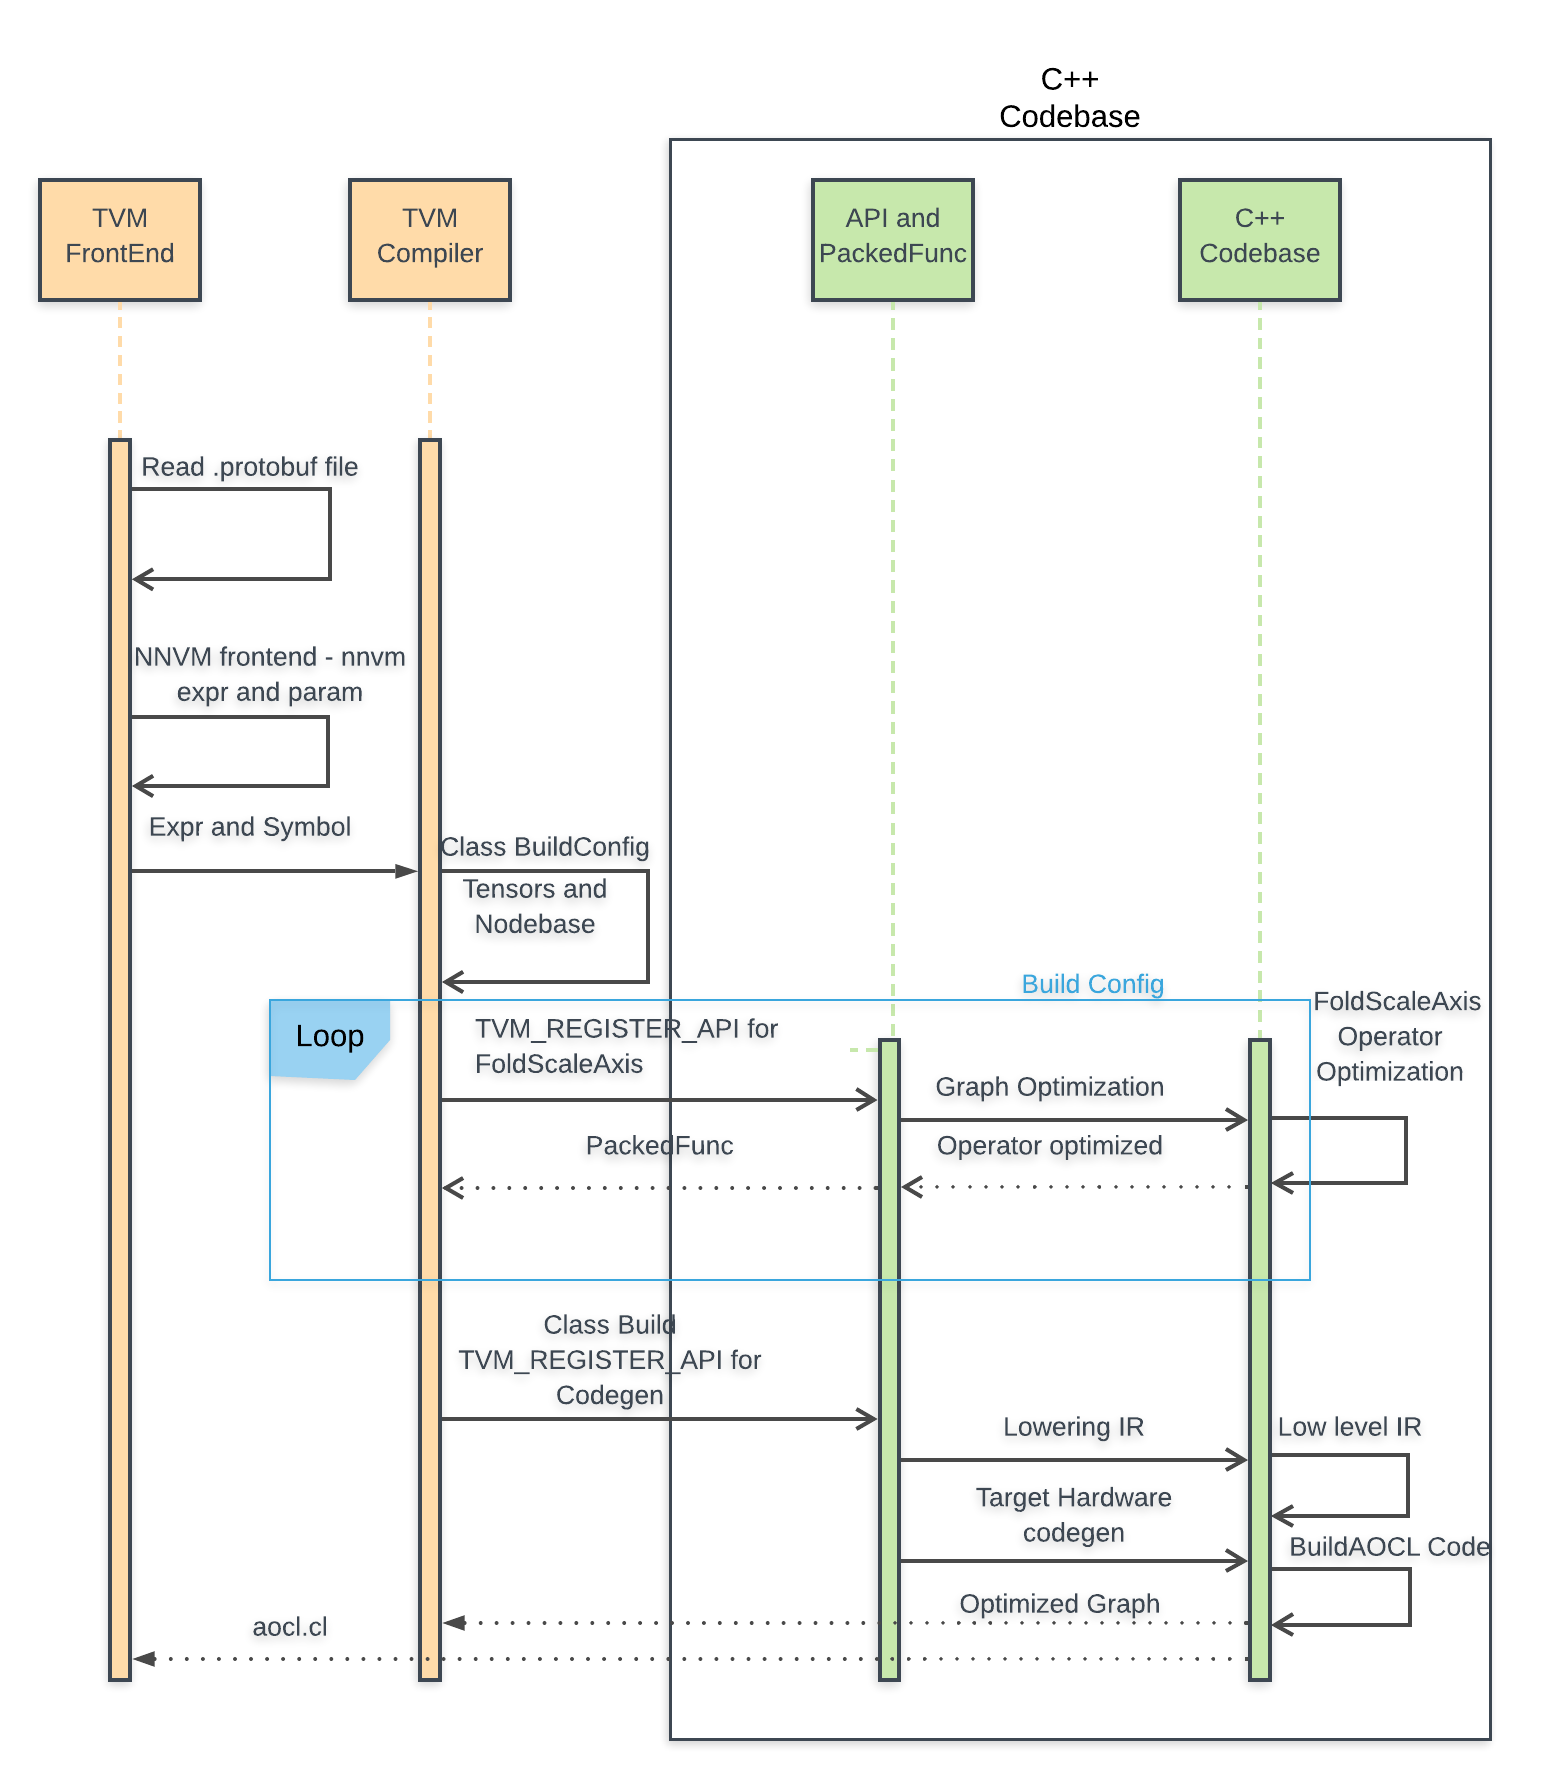
\includegraphics[scale=0.30]{tvm_workflow.png}
    \caption{Sequence diagram of Kernel generation in TVM}
\end{figure}
\pagebreak
 
 \section{Selection of Toolkits}
Reasons for selecting OpenVINO and TVM
 \begin{itemize}
 \item Both Intel OpenVINO and TVM toolkits provide similar features such as Layer fusion, Optimizer, and Quantizer as model optimizer components for optimization of the CNN model. 
 \item We restricted the use of TVM just as OpenCL kernels generator because TVM's AOCL backend for inference was still in experimental phase.
 \item The OpenVINO Inference Engine, as explained earlier comes with several plugins for hardware platforms such as CPU, GPU, FPGA etc. respectively. The FPGA plugin available by default is not open source and works only with certain FPGA boards for which it contains pre-compiled bitstreams. 
 \item Thus, we developed our own FPGA plugin, extending the capabilities of OpenVINO Inference Engine, to make it operational with Stratix 10 FPGAs in the Noctua Cluster of the PC2 infrastructure. 

 \end{itemize}